\documentclass[12pt]{amsart}
\usepackage{amsmath,amsthm,amssymb,amsfonts,enumerate,tikz-cd,fancyhdr}
\openup 5pt
\author[Blake Farman]{Blake Farman\\University of South Carolina}
\title[Exam 02 Solutions]{Math 111\\ Exam 02 Solutions}
\date{November 2, 2017}
\pdfpagewidth 8.5in
\pdfpageheight 11in
\usepackage[margin=1in]{geometry}

\renewcommand{\qedsymbol}{}

\begin{document}
\maketitle

%\theoremstyle{plain}
\theoremstyle{definition}
\newtheorem{thm}{}
\newtheorem{lem}{Lemma}
\newtheorem{defn}{Definition}

\section{Definitions}

\begin{thm}[4 Points]\label{ex1}
  \begin{enumerate}[(a)]
  \item
    State the Point-Slope form of a line passing through the point $(x_0, y_0)$ with slope $m$.
    \begin{proof}[Solution]
      \[y - y_0 = m(x - x_0)\]
    \end{proof}
  \item
    State the Slope-Intercept form of a line with slope $m$ and $y$-intercept $b$.
    \begin{proof}[Solution]
      \[y = mx + b\]
    \end{proof}
  \end{enumerate}
\end{thm}

\begin{thm}[6 Points]\label{ex2}
  Let $f(x)$ be a function.
  State the average rate of change of $f$ between $x = a$ and $x = b$.
\end{thm}

\begin{proof}[Solution]
  \[\frac{f(b) - f(a)}{b - a} = \frac{f(a) - f(b)}{a - b}\]
\end{proof}

\begin{thm}[5 Points]\label{ex3}
  Let $f(x)$ be an exponential function and let $a$ be the growth/decay factor.
  Express the growth/decay rate, $r$, in terms of $a$.
\end{thm}

\begin{proof}[Solution]
  \[r = a - 1\]
\end{proof}

\begin{thm}[3 Points]\label{ex4}
  \begin{enumerate}[(a)]
  \item
    State the general form of an exponential function.
    \begin{proof}[Solution]
      \[Ca^x\]
    \end{proof}
  \item
    When does such a function model exponential growth?
    \begin{proof}[Solution]
      When \(1 < a\).
    \end{proof}
  \item
    When does such a function model exponential decay?
    \begin{proof}[Solution]
      When \(0 < a < 1\).
    \end{proof}
  \end{enumerate}
\end{thm}

\begin{thm}[2 Points]
  Consider the two lines $f(x) = m_1x + b_2$ an $g(x) = m_2x + b_2$.
  \begin{enumerate}[(a)]
  \item
    When are $f$ and $g$ parallel?
    \begin{proof}[Solution]
      When \(m_1 = m_2\).
    \end{proof}
  \item
    When are $f$ and $g$ perpendicular?
    \begin{proof}[Solution]
      When any of the following three equivalent conditions occur
      \begin{itemize}
      \item
        \(\displaystyle{m_1m_2 = -1}\),
      \item
        \(\displaystyle{m_1 = \frac{-1}{m_2}}\), or
      \item
        \(\displaystyle{m_2 = \frac{-1}{m_1}}\).
      \end{itemize}
    \end{proof}
  \end{enumerate}
\end{thm}

\section{Problems}

\begin{thm}[16 Points]\label{ex5}
  In the following problems, use the given information to find the equation of the line in slope-intercept form.
  \begin{enumerate}[(a)]
  \item
    The line passing through the points $(-2,3)$ and $(5,-18)$.
    \begin{proof}[Solution]
      The slope of the line between these points is
      \begin{eqnarray*}
        m &=& \frac{3 - (-18)}{-2 - 5}\\
        &=& \frac{3 + 18}{-7}\\
        &=& -\frac{21}{7}\\
        &=& -3.
      \end{eqnarray*}
      The point-slope form of this line is
      \[y - 3 = -3(x - (-2)) = -3(x + 2)\]
      and the slope-intercept form is
      \[y = -3x - 6 + 3 = -3x - 3\]
    \end{proof}
  \item
    The line passing through the point $(3, -2)$ and parallel to the line $2y - 6x = 8$.
    \begin{proof}[Solution]
      We can put the given line into slope-intercept form by first diving both sides by 2 to get
      \[y - 3x = 4\]
      then adding \(3x\) to both sides to get
      \[y = 3x + 4.\]
      Thus the slope of the parallel line is also \(3\).
      In point-slope form the desired line is
      \[y - (-2) = 3(x - 3).\]
      The slope-intercept form is
      \[ y = 3x - 9 - 2 = 3x - 11.\]
    \end{proof}
  \item
    The line passing through the origin (that is, the point $(0,0)$) and perpendicular to the line $4y - x = 8$.
    \begin{proof}[Solution]
      Adding \(x\) to both sides of the given equation and then dividing both sides by 4 we see that the slope-intercept form of the line is
      \[y = \frac{x}{4} + 8,\]
      so the slope of a perpendicular line is \(-4\).
      Therefore the slope-intercept form of the desired line is
      \[y = -4x.\]
    \end{proof}
  \end{enumerate}
\end{thm}

\begin{thm}[16 Points]\label{ex10}
  Consider the two lines $f(x) = x + 2$ and $g(x) = 3x + 4$.
  Find the point (that is, the $(x,y)$ pair) where these two lines intersect.
\end{thm}

\begin{proof}[Solution]
  To find the point of intersection we need only solve the equation
  $$x + 2 = 3x + 4$$
  for $x$.
  Subtracting $x$ from both sides we get
  \[2 = 2x + 4.\]
  Subtracting 4 from both sides we get
  \[-2 = 2x.\]
  Finally, dividing both sides by 2 we get
  \[x = -1.\]
  The y-coordinate is given by
  \[y = -1 + 2 = 1\]
  so the point of intersection is \((-1,1)\).
\end{proof}

\begin{thm}[16 Points]\label{ex9}
  Let $f(x) = x^2 - 2$.
  \begin{enumerate}[(a)]
  \item
    Compute the average rate of change for $f$ between $x = 2$ and $x = 5$.
    \begin{proof}[Solution]
      The average rate of change is
      \begin{eqnarray*}
        \frac{f(5) - f(2)}{5 - 2} &=& \frac{(25 - 2) - (4 - 2)}{3}\\
        &=& \frac{25 - 2 - 4 + 2}{3}\\
        &=& \frac{25 - 4}{3}\\
        &=& \frac{21}{3}\\
        &=& 7.
      \end{eqnarray*}
    \end{proof}
  \item
    Give the Point-Slope form of the line that passes through $(2, f(2))$ and $(5, f(5))$.
    \begin{proof}[Solution]
      The slope of this line is 7, as computed above.
      The point-slope form of the line is
      \[y - 2 = 7(x - 2).\]
    \end{proof}
  \item
    Give the Slope-Intercept form of the line that passes through $(2, f(2))$ and $(5, f(5))$.
    \begin{proof}[Solution]
      The slope-intercept form of the line is
      \[y = 7x - 14 + 2 = 7x - 12.\]
    \end{proof}
  \end{enumerate}
\end{thm}

\begin{thm}[16 Points]\label{ex7}
  Alice is hosting an event.  She is renting a facility, which costs $\$150$, and providing refreshments, which cost $\$7$ per guest.
  \begin{enumerate}[(a)]
  \item
    Find a function, $C$, that models the total cost of the event if $x$ people attend.
    \begin{proof}[Solution]
      \[C(x) = 7x + 150.\]
    \end{proof}
  \item
    Sketch a graph of $C$.
    \begin{proof}[Solution]
      The function is a line starting from \((0,150)\).
      \begin{center}
        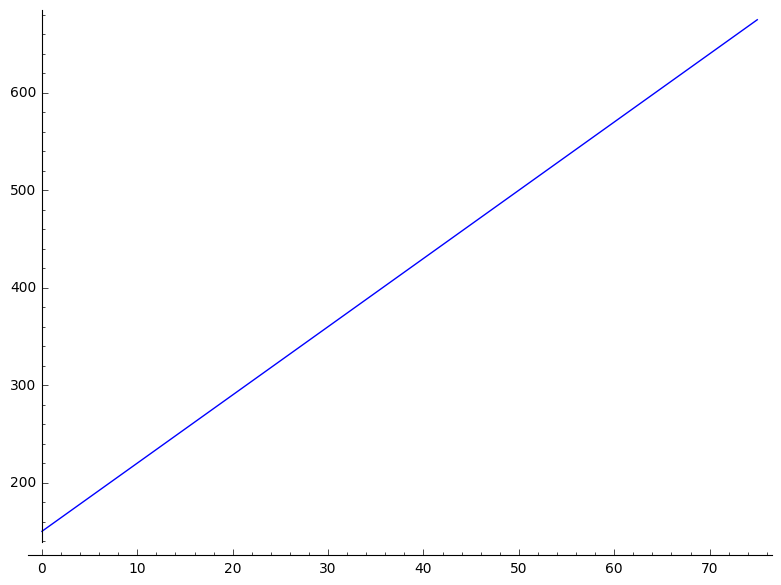
\includegraphics[scale=0.5]{plot.png}
      \end{center}
    \end{proof}
  \item
    Evaluate $C(10)$ and $C(15)$.  What do these numbers represent?
    \begin{proof}[Solution]
      The value
      \[C(10) = 7(10) + 150 = 70 + 150 = 220\]
      represents the cost if 10 people attend and the value
      \[C(15) = 7(15) + 150 = 105 + 150 = 255\]
      represents the cost if 15 people attend.
    \end{proof}
  \item
    If the total cost for the event was $\$500$, how many people attended?
    \begin{proof}[Solution]
      To find the number of people that attended the party, solve
      \[500 = C(x) = 7x + 150\]
      for $x$.
      The solution is given by subtracting 150 from both sides of the equation then dividing both sides of the equation by 7, so
      \[x = \frac{500 - 150}{7} = \frac{350}{7} = 50.\]
      Therefore 50 people attended.
    \end{proof}
  \end{enumerate}
\end{thm}

\begin{thm}[16 Points]
  A population of size $32$ grows by $25\%$ every day.
  \begin{enumerate}[(a)]
  \item
    Give the daily growth factor for this population.
    \begin{proof}[Solution]
      We are given the daily growth rate
      $$r = 25\% = \frac{25}{100} = \frac{25}{4(25)} = \frac{1}{4}$$
      so the daily growth factor is given by
      \[a = 1 + r = 1 + \frac{1}{4} = \frac{4}{4} + \frac{1}{4} = \frac{5}{4}.\]
    \end{proof}
  \item
    Give an exponential model for the size of the population after $t$ days.
    \begin{proof}[Solution]
      The population is modeled by
      \[P(t) = 32\left(\frac{5}{4}\right)^t.\]
    \end{proof}
  \item
    Determine the size of the population after 2 days.
    
    \noindent[Hint: Express the growth factor as a fraction, rather than a decimal, and this will be very easy to compute.]
    \begin{proof}[Solution]
      The population after 2 days is
      \[P(2) = 32\left(\frac{5}{4}\right)^2 = 32\left(\frac{5^2}{4^2}\right)= 32\left(\frac{25}{16}\right) = 2(25) = 50.\]
    \end{proof}
  \end{enumerate}
\end{thm}

%\newpage

%\begin{thm}[Bonus - 5 Points]\label{bonus}
%  Let $f(x) = x^2 - 1$.
%  Show that the average rate of change of $f$ between $x = a$ and $x = b$ is always $a + b$.
%\end{thm}

\end{document}
